\documentclass[twoside]{book}

% Packages required by doxygen
\usepackage{fixltx2e}
\usepackage{calc}
\usepackage{doxygen}
\usepackage{graphicx}
\usepackage[utf8]{inputenc}
\usepackage{makeidx}
\usepackage{multicol}
\usepackage{multirow}
\PassOptionsToPackage{warn}{textcomp}
\usepackage{textcomp}
\usepackage[nointegrals]{wasysym}
\usepackage[table]{xcolor}

% Font selection
\usepackage[T1]{fontenc}
\usepackage{mathptmx}
\usepackage[scaled=.90]{helvet}
\usepackage{courier}
\usepackage{amssymb}
\usepackage{sectsty}
\renewcommand{\familydefault}{\sfdefault}
\allsectionsfont{%
  \fontseries{bc}\selectfont%
  \color{darkgray}%
}
\renewcommand{\DoxyLabelFont}{%
  \fontseries{bc}\selectfont%
  \color{darkgray}%
}
\newcommand{\+}{\discretionary{\mbox{\scriptsize$\hookleftarrow$}}{}{}}

% Page & text layout
\usepackage{geometry}
\geometry{%
  a4paper,%
  top=2.5cm,%
  bottom=2.5cm,%
  left=2.5cm,%
  right=2.5cm%
}
\tolerance=750
\hfuzz=15pt
\hbadness=750
\setlength{\emergencystretch}{15pt}
\setlength{\parindent}{0cm}
\setlength{\parskip}{0.2cm}
\makeatletter
\renewcommand{\paragraph}{%
  \@startsection{paragraph}{4}{0ex}{-1.0ex}{1.0ex}{%
    \normalfont\normalsize\bfseries\SS@parafont%
  }%
}
\renewcommand{\subparagraph}{%
  \@startsection{subparagraph}{5}{0ex}{-1.0ex}{1.0ex}{%
    \normalfont\normalsize\bfseries\SS@subparafont%
  }%
}
\makeatother

% Headers & footers
\usepackage{fancyhdr}
\pagestyle{fancyplain}
\fancyhead[LE]{\fancyplain{}{\bfseries\thepage}}
\fancyhead[CE]{\fancyplain{}{}}
\fancyhead[RE]{\fancyplain{}{\bfseries\leftmark}}
\fancyhead[LO]{\fancyplain{}{\bfseries\rightmark}}
\fancyhead[CO]{\fancyplain{}{}}
\fancyhead[RO]{\fancyplain{}{\bfseries\thepage}}
\fancyfoot[LE]{\fancyplain{}{}}
\fancyfoot[CE]{\fancyplain{}{}}
\fancyfoot[RE]{\fancyplain{}{\bfseries\scriptsize Generated on Thu Sep 29 2016 22\+:30\+:28 for My Project by Doxygen }}
\fancyfoot[LO]{\fancyplain{}{\bfseries\scriptsize Generated on Thu Sep 29 2016 22\+:30\+:28 for My Project by Doxygen }}
\fancyfoot[CO]{\fancyplain{}{}}
\fancyfoot[RO]{\fancyplain{}{}}
\renewcommand{\footrulewidth}{0.4pt}
\renewcommand{\chaptermark}[1]{%
  \markboth{#1}{}%
}
\renewcommand{\sectionmark}[1]{%
  \markright{\thesection\ #1}%
}

% Indices & bibliography
\usepackage{natbib}
\usepackage[titles]{tocloft}
\setcounter{tocdepth}{3}
\setcounter{secnumdepth}{5}
\makeindex

% Hyperlinks (required, but should be loaded last)
\usepackage{ifpdf}
\ifpdf
  \usepackage[pdftex,pagebackref=true]{hyperref}
\else
  \usepackage[ps2pdf,pagebackref=true]{hyperref}
\fi
\hypersetup{%
  colorlinks=true,%
  linkcolor=blue,%
  citecolor=blue,%
  unicode%
}

% Custom commands
\newcommand{\clearemptydoublepage}{%
  \newpage{\pagestyle{empty}\cleardoublepage}%
}


%===== C O N T E N T S =====

\begin{document}

% Titlepage & ToC
\hypersetup{pageanchor=false,
             bookmarks=true,
             bookmarksnumbered=true,
             pdfencoding=unicode
            }
\pagenumbering{roman}
\begin{titlepage}
\vspace*{7cm}
\begin{center}%
{\Large My Project }\\
\vspace*{1cm}
{\large Generated by Doxygen 1.8.8}\\
\vspace*{0.5cm}
{\small Thu Sep 29 2016 22:30:28}\\
\end{center}
\end{titlepage}
\clearemptydoublepage
\tableofcontents
\clearemptydoublepage
\pagenumbering{arabic}
\hypersetup{pageanchor=true}

%--- Begin generated contents ---
\chapter{Class Index}
\section{Class List}
Here are the classes, structs, unions and interfaces with brief descriptions\+:\begin{DoxyCompactList}
\item\contentsline{section}{\hyperlink{class_juego_de_la_vida}{Juego\+De\+La\+Vida} }{\pageref{class_juego_de_la_vida}}{}
\end{DoxyCompactList}

\chapter{Class Documentation}
\hypertarget{class_calculadora}{\section{Calculadora$<$ T $>$ Class Template Reference}
\label{class_calculadora}\index{Calculadora$<$ T $>$@{Calculadora$<$ T $>$}}
}


Collaboration diagram for Calculadora$<$ T $>$\+:
\nopagebreak
\begin{figure}[H]
\begin{center}
\leavevmode
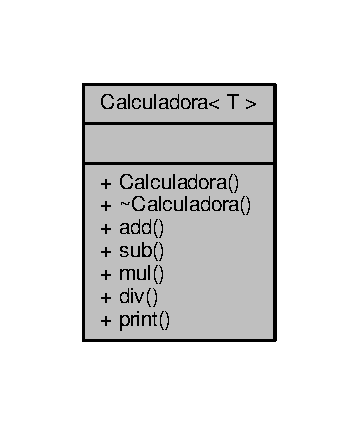
\includegraphics[width=172pt]{class_calculadora__coll__graph}
\end{center}
\end{figure}
\subsection*{Public Member Functions}
\begin{DoxyCompactItemize}
\item 
\hypertarget{class_calculadora_a385159b71410804ebe0daa54d7e05d1e}{\hyperlink{class_calculadora_a385159b71410804ebe0daa54d7e05d1e}{Calculadora} ()}\label{class_calculadora_a385159b71410804ebe0daa54d7e05d1e}

\begin{DoxyCompactList}\small\item\em Constructor vacío de \hyperlink{class_calculadora}{Calculadora}. \end{DoxyCompactList}\item 
\hypertarget{class_calculadora_a9a59d0072fd27163625e14ab90d9ad1e}{virtual \hyperlink{class_calculadora_a9a59d0072fd27163625e14ab90d9ad1e}{$\sim$\+Calculadora} ()}\label{class_calculadora_a9a59d0072fd27163625e14ab90d9ad1e}

\begin{DoxyCompactList}\small\item\em Destructor de \hyperlink{class_calculadora}{Calculadora}. \end{DoxyCompactList}\item 
\hypertarget{class_calculadora_a648f902edf66a0fc1e17469d3fa61471}{T \hyperlink{class_calculadora_a648f902edf66a0fc1e17469d3fa61471}{add} (T a, const T b)}\label{class_calculadora_a648f902edf66a0fc1e17469d3fa61471}

\begin{DoxyCompactList}\small\item\em Función suma de \hyperlink{class_calculadora}{Calculadora}. \end{DoxyCompactList}\item 
\hypertarget{class_calculadora_ae92d8eb0a75b146167bebcfbbc2b0bfd}{T \hyperlink{class_calculadora_ae92d8eb0a75b146167bebcfbbc2b0bfd}{sub} (T a, const T b)}\label{class_calculadora_ae92d8eb0a75b146167bebcfbbc2b0bfd}

\begin{DoxyCompactList}\small\item\em Función resta de \hyperlink{class_calculadora}{Calculadora}. \end{DoxyCompactList}\item 
\hypertarget{class_calculadora_a88b22c85e262aa507630f03e77a6c066}{T \hyperlink{class_calculadora_a88b22c85e262aa507630f03e77a6c066}{mul} (T a, const T b)}\label{class_calculadora_a88b22c85e262aa507630f03e77a6c066}

\begin{DoxyCompactList}\small\item\em Función multiplicación de \hyperlink{class_calculadora}{Calculadora}. \end{DoxyCompactList}\item 
\hypertarget{class_calculadora_a38b613e1d241ec59744420fb49267920}{T \hyperlink{class_calculadora_a38b613e1d241ec59744420fb49267920}{div} (T a, const T b)}\label{class_calculadora_a38b613e1d241ec59744420fb49267920}

\begin{DoxyCompactList}\small\item\em Función división de \hyperlink{class_calculadora}{Calculadora}. \end{DoxyCompactList}\item 
\hypertarget{class_calculadora_a6cb0a45ce2942e41fe802183b918fe87}{void \hyperlink{class_calculadora_a6cb0a45ce2942e41fe802183b918fe87}{print} (const T a)}\label{class_calculadora_a6cb0a45ce2942e41fe802183b918fe87}

\begin{DoxyCompactList}\small\item\em Función imprimir de alculadora. \end{DoxyCompactList}\end{DoxyCompactItemize}


The documentation for this class was generated from the following file\+:\begin{DoxyCompactItemize}
\item 
Calculadora.\+h\end{DoxyCompactItemize}

\hypertarget{class_fraccion}{\section{Fraccion Class Reference}
\label{class_fraccion}\index{Fraccion@{Fraccion}}
}


Collaboration diagram for Fraccion\+:
\nopagebreak
\begin{figure}[H]
\begin{center}
\leavevmode
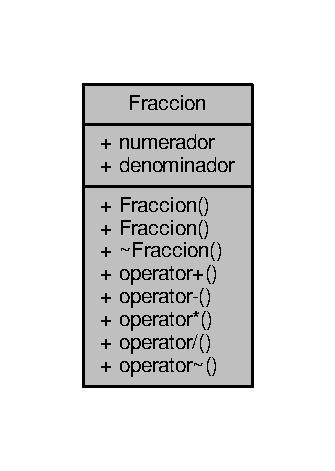
\includegraphics[width=161pt]{class_fraccion__coll__graph}
\end{center}
\end{figure}
\subsection*{Public Member Functions}
\begin{DoxyCompactItemize}
\item 
\hypertarget{class_fraccion_a80b8bb475192ceb820428a57e911ceb5}{\hyperlink{class_fraccion_a80b8bb475192ceb820428a57e911ceb5}{Fraccion} ()}\label{class_fraccion_a80b8bb475192ceb820428a57e911ceb5}

\begin{DoxyCompactList}\small\item\em Constructor vacío de \hyperlink{class_fraccion}{Fraccion}. \end{DoxyCompactList}\item 
\hypertarget{class_fraccion_a6f9e2752a686e2508b94f33cbdc9ab15}{\hyperlink{class_fraccion_a6f9e2752a686e2508b94f33cbdc9ab15}{Fraccion} (int \hyperlink{class_fraccion_a88946835a0fe344bf223ac98e23f4e4a}{numerador}, int denominador)}\label{class_fraccion_a6f9e2752a686e2508b94f33cbdc9ab15}

\begin{DoxyCompactList}\small\item\em Constructor de \hyperlink{class_fraccion}{Fraccion}. \end{DoxyCompactList}\item 
\hypertarget{class_fraccion_abb2ec579092e5bc50e7c3644ea718084}{virtual \hyperlink{class_fraccion_abb2ec579092e5bc50e7c3644ea718084}{$\sim$\+Fraccion} ()}\label{class_fraccion_abb2ec579092e5bc50e7c3644ea718084}

\begin{DoxyCompactList}\small\item\em Destructor de \hyperlink{class_fraccion}{Fraccion}. \end{DoxyCompactList}\item 
\hyperlink{class_fraccion}{Fraccion} \hyperlink{class_fraccion_a5aa3438285f57e1ccce0aa2f1602bd26}{operator+} (const \hyperlink{class_fraccion}{Fraccion} \&)
\begin{DoxyCompactList}\small\item\em Funciones de \hyperlink{class_fraccion}{Fraccion}. \end{DoxyCompactList}\item 
\hypertarget{class_fraccion_a3844e2c49a0439d19495064cf138e857}{\hyperlink{class_fraccion}{Fraccion} \hyperlink{class_fraccion_a3844e2c49a0439d19495064cf138e857}{operator-\/} (const \hyperlink{class_fraccion}{Fraccion} \&)}\label{class_fraccion_a3844e2c49a0439d19495064cf138e857}

\begin{DoxyCompactList}\small\item\em Resta de \hyperlink{class_fraccion}{Fraccion}. \end{DoxyCompactList}\item 
\hypertarget{class_fraccion_ab6634c35da9689efe4e99a190317d5a2}{\hyperlink{class_fraccion}{Fraccion} \hyperlink{class_fraccion_ab6634c35da9689efe4e99a190317d5a2}{operator$\ast$} (const \hyperlink{class_fraccion}{Fraccion} \&)}\label{class_fraccion_ab6634c35da9689efe4e99a190317d5a2}

\begin{DoxyCompactList}\small\item\em Multiplicación de \hyperlink{class_fraccion}{Fraccion}. \end{DoxyCompactList}\item 
\hypertarget{class_fraccion_a02cbdcc3a8086bc19c3e5f3372e316b5}{\hyperlink{class_fraccion}{Fraccion} \hyperlink{class_fraccion_a02cbdcc3a8086bc19c3e5f3372e316b5}{operator/} (const \hyperlink{class_fraccion}{Fraccion} \&)}\label{class_fraccion_a02cbdcc3a8086bc19c3e5f3372e316b5}

\begin{DoxyCompactList}\small\item\em División de \hyperlink{class_fraccion}{Fraccion}. \end{DoxyCompactList}\item 
\hypertarget{class_fraccion_a6ba2dac78e5ef60d6860d39ba3489bb1}{void \hyperlink{class_fraccion_a6ba2dac78e5ef60d6860d39ba3489bb1}{operator$\sim$} ()}\label{class_fraccion_a6ba2dac78e5ef60d6860d39ba3489bb1}

\begin{DoxyCompactList}\small\item\em Función imprimir de \hyperlink{class_fraccion}{Fraccion} (sobrecarga del operador $\sim$) \end{DoxyCompactList}\end{DoxyCompactItemize}
\subsection*{Public Attributes}
\begin{DoxyCompactItemize}
\item 
\hypertarget{class_fraccion_a88946835a0fe344bf223ac98e23f4e4a}{int \hyperlink{class_fraccion_a88946835a0fe344bf223ac98e23f4e4a}{numerador}}\label{class_fraccion_a88946835a0fe344bf223ac98e23f4e4a}

\begin{DoxyCompactList}\small\item\em Atributos de \hyperlink{class_fraccion}{Fraccion}. \end{DoxyCompactList}\item 
\hypertarget{class_fraccion_a3857a3268d25091dcb00decf4d4516cd}{int {\bfseries denominador}}\label{class_fraccion_a3857a3268d25091dcb00decf4d4516cd}

\end{DoxyCompactItemize}


\subsection{Member Function Documentation}
\hypertarget{class_fraccion_a5aa3438285f57e1ccce0aa2f1602bd26}{\index{Fraccion@{Fraccion}!operator+@{operator+}}
\index{operator+@{operator+}!Fraccion@{Fraccion}}
\subsubsection[{operator+}]{\setlength{\rightskip}{0pt plus 5cm}{\bf Fraccion} Fraccion\+::operator+ (
\begin{DoxyParamCaption}
\item[{const {\bf Fraccion} \&}]{other}
\end{DoxyParamCaption}
)}}\label{class_fraccion_a5aa3438285f57e1ccce0aa2f1602bd26}


Funciones de \hyperlink{class_fraccion}{Fraccion}. 

Suma de \hyperlink{class_fraccion}{Fraccion}. 

The documentation for this class was generated from the following files\+:\begin{DoxyCompactItemize}
\item 
Fraccion.\+h\item 
Fraccion.\+cpp\end{DoxyCompactItemize}

\hypertarget{class_matriz}{\section{Matriz Class Reference}
\label{class_matriz}\index{Matriz@{Matriz}}
}


Collaboration diagram for Matriz\+:
\nopagebreak
\begin{figure}[H]
\begin{center}
\leavevmode
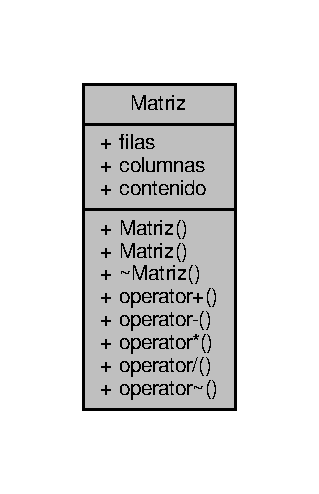
\includegraphics[width=153pt]{class_matriz__coll__graph}
\end{center}
\end{figure}
\subsection*{Public Member Functions}
\begin{DoxyCompactItemize}
\item 
\hypertarget{class_matriz_a7de756301bddbc4b0b5d2a0f2b1fc695}{\hyperlink{class_matriz_a7de756301bddbc4b0b5d2a0f2b1fc695}{Matriz} ()}\label{class_matriz_a7de756301bddbc4b0b5d2a0f2b1fc695}

\begin{DoxyCompactList}\small\item\em Constructor vacío de \hyperlink{class_matriz}{Matriz}. \end{DoxyCompactList}\item 
\hypertarget{class_matriz_a9042b03b0030c81bc2d6acd3e90c3168}{\hyperlink{class_matriz_a9042b03b0030c81bc2d6acd3e90c3168}{Matriz} (int \hyperlink{class_matriz_a0696de23c471bd7b02c3724aa007276d}{filas}, int columnas, int $\ast$$\ast$contenido)}\label{class_matriz_a9042b03b0030c81bc2d6acd3e90c3168}

\begin{DoxyCompactList}\small\item\em Constructor de \hyperlink{class_matriz}{Matriz}. \end{DoxyCompactList}\item 
\hypertarget{class_matriz_a2092b7a289ecec369e1da407d5839f5a}{virtual \hyperlink{class_matriz_a2092b7a289ecec369e1da407d5839f5a}{$\sim$\+Matriz} ()}\label{class_matriz_a2092b7a289ecec369e1da407d5839f5a}

\begin{DoxyCompactList}\small\item\em Destructor de \hyperlink{class_matriz}{Matriz}. \end{DoxyCompactList}\item 
\hyperlink{class_matriz}{Matriz} \hyperlink{class_matriz_a3b34427eff71649f3611a9e6a5630f5e}{operator+} (const \hyperlink{class_matriz}{Matriz} \&)
\begin{DoxyCompactList}\small\item\em Funciones de \hyperlink{class_matriz}{Matriz}. \end{DoxyCompactList}\item 
\hypertarget{class_matriz_a582dd920be1081172511c6eeb941201f}{\hyperlink{class_matriz}{Matriz} \hyperlink{class_matriz_a582dd920be1081172511c6eeb941201f}{operator-\/} (const \hyperlink{class_matriz}{Matriz} \&)}\label{class_matriz_a582dd920be1081172511c6eeb941201f}

\begin{DoxyCompactList}\small\item\em Función resta de \hyperlink{class_matriz}{Matriz}. \end{DoxyCompactList}\item 
\hypertarget{class_matriz_a32f350fb2091ff6ee3ad7ca9135a7e4e}{\hyperlink{class_matriz}{Matriz} {\bfseries operator$\ast$} (const \hyperlink{class_matriz}{Matriz} \&)}\label{class_matriz_a32f350fb2091ff6ee3ad7ca9135a7e4e}

\item 
\hypertarget{class_matriz_a3757454cd8555a964805200b87ccff6f}{\hyperlink{class_matriz}{Matriz} \hyperlink{class_matriz_a3757454cd8555a964805200b87ccff6f}{operator/} (const \hyperlink{class_matriz}{Matriz} \&)}\label{class_matriz_a3757454cd8555a964805200b87ccff6f}

\begin{DoxyCompactList}\small\item\em Función división de \hyperlink{class_matriz}{Matriz}. \end{DoxyCompactList}\item 
\hypertarget{class_matriz_a7eb9064958c359ce2f6b6ab0327b1282}{void \hyperlink{class_matriz_a7eb9064958c359ce2f6b6ab0327b1282}{operator$\sim$} ()}\label{class_matriz_a7eb9064958c359ce2f6b6ab0327b1282}

\begin{DoxyCompactList}\small\item\em Función imprimir de \hyperlink{class_matriz}{Matriz} (sobrecarga del operador $\sim$) \end{DoxyCompactList}\end{DoxyCompactItemize}
\subsection*{Public Attributes}
\begin{DoxyCompactItemize}
\item 
\hypertarget{class_matriz_a0696de23c471bd7b02c3724aa007276d}{int \hyperlink{class_matriz_a0696de23c471bd7b02c3724aa007276d}{filas}}\label{class_matriz_a0696de23c471bd7b02c3724aa007276d}

\begin{DoxyCompactList}\small\item\em Atributos de \hyperlink{class_matriz}{Matriz}. \end{DoxyCompactList}\item 
\hypertarget{class_matriz_a7c034f5eb81585a62ac1331c2127ac19}{int {\bfseries columnas}}\label{class_matriz_a7c034f5eb81585a62ac1331c2127ac19}

\item 
\hypertarget{class_matriz_a5cc3d2e7d7b29fab5c395ad022446a7e}{int $\ast$$\ast$ {\bfseries contenido}}\label{class_matriz_a5cc3d2e7d7b29fab5c395ad022446a7e}

\end{DoxyCompactItemize}


\subsection{Member Function Documentation}
\hypertarget{class_matriz_a3b34427eff71649f3611a9e6a5630f5e}{\index{Matriz@{Matriz}!operator+@{operator+}}
\index{operator+@{operator+}!Matriz@{Matriz}}
\subsubsection[{operator+}]{\setlength{\rightskip}{0pt plus 5cm}{\bf Matriz} Matriz\+::operator+ (
\begin{DoxyParamCaption}
\item[{const {\bf Matriz} \&}]{other}
\end{DoxyParamCaption}
)}}\label{class_matriz_a3b34427eff71649f3611a9e6a5630f5e}


Funciones de \hyperlink{class_matriz}{Matriz}. 

Función suma de \hyperlink{class_matriz}{Matriz}. 

The documentation for this class was generated from the following files\+:\begin{DoxyCompactItemize}
\item 
Matriz.\+h\item 
Matriz.\+cpp\end{DoxyCompactItemize}

\hypertarget{class_polinomio}{\section{Polinomio Class Reference}
\label{class_polinomio}\index{Polinomio@{Polinomio}}
}


Collaboration diagram for Polinomio\+:
\nopagebreak
\begin{figure}[H]
\begin{center}
\leavevmode
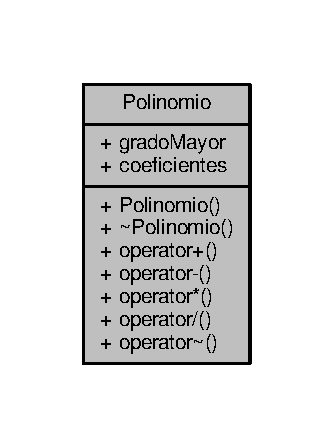
\includegraphics[width=160pt]{class_polinomio__coll__graph}
\end{center}
\end{figure}
\subsection*{Public Member Functions}
\begin{DoxyCompactItemize}
\item 
\hyperlink{class_polinomio_a952907e68bab3276d0688dde766c26b1}{Polinomio} (int \hyperlink{class_polinomio_a42b14d0901152a448b86808fd438382b}{grado\+Mayor}, int $\ast$coeficientes)
\begin{DoxyCompactList}\small\item\em Constructor vacío de \hyperlink{class_polinomio}{Polinomio}. \end{DoxyCompactList}\item 
\hypertarget{class_polinomio_a1023ada36c95fce6698316a632fdcc1c}{virtual \hyperlink{class_polinomio_a1023ada36c95fce6698316a632fdcc1c}{$\sim$\+Polinomio} ()}\label{class_polinomio_a1023ada36c95fce6698316a632fdcc1c}

\begin{DoxyCompactList}\small\item\em Destructor de \hyperlink{class_polinomio}{Polinomio}. \end{DoxyCompactList}\item 
\hyperlink{class_polinomio}{Polinomio} \hyperlink{class_polinomio_ac6cdcb7a9b33ad0f4c7fed22bc665afa}{operator+} (const \hyperlink{class_polinomio}{Polinomio} \&other)
\begin{DoxyCompactList}\small\item\em Funciones de \hyperlink{class_polinomio}{Polinomio}. \end{DoxyCompactList}\item 
\hypertarget{class_polinomio_a83f1bb909fa1adfdba0325e693bc0e6a}{\hyperlink{class_polinomio}{Polinomio} \hyperlink{class_polinomio_a83f1bb909fa1adfdba0325e693bc0e6a}{operator-\/} (const \hyperlink{class_polinomio}{Polinomio} \&other)}\label{class_polinomio_a83f1bb909fa1adfdba0325e693bc0e6a}

\begin{DoxyCompactList}\small\item\em Función resta de Polinomios (sobrecarga de operador -\/) \end{DoxyCompactList}\item 
\hypertarget{class_polinomio_a3a604e2ef650894fb3cdc2b215f512b7}{\hyperlink{class_polinomio}{Polinomio} \hyperlink{class_polinomio_a3a604e2ef650894fb3cdc2b215f512b7}{operator$\ast$} (const \hyperlink{class_polinomio}{Polinomio} \&other)}\label{class_polinomio_a3a604e2ef650894fb3cdc2b215f512b7}

\begin{DoxyCompactList}\small\item\em Funcion multiplicar Polinomios (sobrecarga de operadorb $\ast$) \end{DoxyCompactList}\item 
\hypertarget{class_polinomio_a7015af39ddcf8a94b6253ab469ff3761}{\hyperlink{class_polinomio}{Polinomio} \hyperlink{class_polinomio_a7015af39ddcf8a94b6253ab469ff3761}{operator/} (const \hyperlink{class_polinomio}{Polinomio} \&other)}\label{class_polinomio_a7015af39ddcf8a94b6253ab469ff3761}

\begin{DoxyCompactList}\small\item\em Funcion dividir Polinomios (sobrecarga de operador $\ast$) \end{DoxyCompactList}\item 
\hypertarget{class_polinomio_a3433445a715a473c4dd433e1d1248406}{void \hyperlink{class_polinomio_a3433445a715a473c4dd433e1d1248406}{operator$\sim$} ()}\label{class_polinomio_a3433445a715a473c4dd433e1d1248406}

\begin{DoxyCompactList}\small\item\em Función imprimir de \hyperlink{class_polinomio}{Polinomio} (sobrecarga del operador $\sim$) \end{DoxyCompactList}\end{DoxyCompactItemize}
\subsection*{Public Attributes}
\begin{DoxyCompactItemize}
\item 
\hypertarget{class_polinomio_a42b14d0901152a448b86808fd438382b}{int \hyperlink{class_polinomio_a42b14d0901152a448b86808fd438382b}{grado\+Mayor}}\label{class_polinomio_a42b14d0901152a448b86808fd438382b}

\begin{DoxyCompactList}\small\item\em Atributos de \hyperlink{class_polinomio}{Polinomio}. \end{DoxyCompactList}\item 
\hypertarget{class_polinomio_ae55bb8ffc2984a1a156ebc58380e1e71}{int $\ast$ {\bfseries coeficientes}}\label{class_polinomio_ae55bb8ffc2984a1a156ebc58380e1e71}

\end{DoxyCompactItemize}


\subsection{Constructor \& Destructor Documentation}
\hypertarget{class_polinomio_a952907e68bab3276d0688dde766c26b1}{\index{Polinomio@{Polinomio}!Polinomio@{Polinomio}}
\index{Polinomio@{Polinomio}!Polinomio@{Polinomio}}
\subsubsection[{Polinomio}]{\setlength{\rightskip}{0pt plus 5cm}Polinomio\+::\+Polinomio (
\begin{DoxyParamCaption}
\item[{int}]{grado\+Mayor, }
\item[{int $\ast$}]{coeficientes}
\end{DoxyParamCaption}
)}}\label{class_polinomio_a952907e68bab3276d0688dde766c26b1}


Constructor vacío de \hyperlink{class_polinomio}{Polinomio}. 

Constructor de \hyperlink{class_polinomio}{Polinomio}.

Constructor de \hyperlink{class_polinomio}{Polinomio} 

\subsection{Member Function Documentation}
\hypertarget{class_polinomio_ac6cdcb7a9b33ad0f4c7fed22bc665afa}{\index{Polinomio@{Polinomio}!operator+@{operator+}}
\index{operator+@{operator+}!Polinomio@{Polinomio}}
\subsubsection[{operator+}]{\setlength{\rightskip}{0pt plus 5cm}{\bf Polinomio} Polinomio\+::operator+ (
\begin{DoxyParamCaption}
\item[{const {\bf Polinomio} \&}]{other}
\end{DoxyParamCaption}
)}}\label{class_polinomio_ac6cdcb7a9b33ad0f4c7fed22bc665afa}


Funciones de \hyperlink{class_polinomio}{Polinomio}. 

Función de suma de \hyperlink{class_polinomio}{Polinomio} (sobrecarga del operador +) 

The documentation for this class was generated from the following files\+:\begin{DoxyCompactItemize}
\item 
Polinomio.\+h\item 
Polinomio.\+cpp\end{DoxyCompactItemize}

%--- End generated contents ---

% Index
\newpage
\phantomsection
\addcontentsline{toc}{chapter}{Index}
\printindex

\end{document}
